% cd ..\..\Users\NikitaSkybytskyi\Desktop\eco\labs\examples\3\tex
% cls && pdflatex report.tex && cls && pdflatex report.tex && del report.aux, report.toc, report.log, report.out && start report.pdf
\documentclass[12pt, a4paper]{article}
\usepackage[T2A]{fontenc}
\usepackage[utf8]{inputenc}
\usepackage[english,ukrainian]{babel}
\usepackage{amsmath, amssymb}

\usepackage[top = 2 cm, left = 1 cm, right = 1 cm, bottom = 2 cm]{geometry}

\usepackage{float, graphicx}

\usepackage{minted}

\newcommand*\diff{\mathop{}\!\mathrm{d}}

\setlength\parindent{0pt}
\allowdisplaybreaks

\newcommand{\cover}[2]{
	\begin{center}
	\hfill \break
		Міністерство освіти та науки України \\
		Київський національний університет імені Тараса Шевченка \\ 
		Факультет комп'ютерних наук та кібернетики \\
		Кафедра обчислювальної математики
	\end{center}

	\vfill 

	\begin{center}
		\large{
			Звіт до лабораторної роботи №{#1} на тему: \\ 
			``{#2}''
		}
	\end{center}

	\vfill 

	\begin{flushright}
		Виконав студент групи ОМ-3 \\
		Скибицький Нікіта
	\end{flushright}

	\vfill 

	\begin{center}
	    Київ, 2019
	\end{center}

	\thispagestyle{empty} 
	\newpage
}

\begin{document}

\cover{3}{Попит та пропозиція. Ринкова рівновага. \\ Стабільність рівноваги. Вплив дотації}

\tableofcontents

\section{Теоретичні відомості}

\subsection{Аналітична апроксимація}

За заданою таблицею значень попиту $d_i$ і пропозиції $s_i$ в залежності від ціни $p_i$, $i = \overline{1, n}$ знаходиться аналітичний вигляд функцій $Q_d(P)$ та $Q_s(P)$. \medskip

Наприклад, можна обмежитися певною сім'єю параметризованих функцій, наприклад \[ Q_d(P) = a_d \cdot P + b_p, \] тобто лінійних функцій, або \[ Q_s(P) = a_s \cdot \exp\left\{b_s \cdot P\right\}, \] тобто експонент. Серед найрозповсюдженіших моделей залежностей можна також виділити логарифмічну, тобто \[ y = a + b \cdot \ln(x) \] і поліноміальну, тобто \[ y = a_0 + a_1 x + \ldots + a_n x^n. \]

Таке обмеження дозволяє поставити скінченно-вимірну оптимізаційну задачу \[ \mathcal{J}(Q_d) = \sum_{i = 1}^n \left( Q_d(p_i) - d_i \right)^2 \to \min, \] розв'язок знаходиться за допомогою ітераційних чисельних або навіть аналітичних методів (у випадку найпростіших моделей). \medskip

Рекомендується не одразу обмежуватися лише одним класом залежностей, а спробувати усі найпоширеніші, знайти оптимальну функцію з кожного класу, обчислити для них середньоквадратичні відхилення і обирати той клас, на якому досягається мінімум середньоквадратичного відхилення.

\subsection{Стабільність рівноваги}

За знайденими аналітичними виглядами функці $Q_d(P)$ та $Q_s(P)$ будються графіки, спочатку у вісях $(P, Q)$ (для математиків), а згодом і у $(Q, P)$ (для економістів), знаходиться точка ринкової рівноваги $(P^\star, Q^\star)$ у якій \[ Q_s(P^\star) = Q_d(P^\star) = Q^\star. \]

Ринок рідко перебуває саме у стані рівноваги, здебільшого відбувається покрокове ітеративне уточнення ціни $P$ (і, як наслідок, обсягу $Q$), причому в залежності від поведінки функцій $Q_s(\cdot)$ та $Q_d(\cdot)$ в околі точки $(P^\star, Q^\star)$ залижть чи ринок прямує до стану рівноваги, чи він осцилює довкола, чи навіть віддаляється. \medskip

Поведінка ринку залежить від стабільності точки рівноваги, яка може бути виражена у числах наступним чином:
\begin{itemize}
	\item Якщо $\left. \left| \dfrac{\diff Q_d}{\diff P} \right| \right|_{P = P^\star} > \left. \dfrac{\diff Q_s}{\diff P} \right|_{P = P^\star}$, то рівновага стійка.
	\item Якщо $\left. \left| \dfrac{\diff Q_d}{\diff P} \right| \right|_{P = P^\star} = \left. \dfrac{\diff Q_s}{\diff P} \right|_{P = P^\star}$, то відбуваються коливання довкола рівноваги.
	\item Якщо $\left. \left| \dfrac{\diff Q_d}{\diff P} \right| \right|_{P = P^\star} < \left. \dfrac{\diff Q_s}{\diff P} \right|_{P = P^\star}$, то рівновага не стійка.
\end{itemize}

\subsection{Вплив державного регулювання}

Існує щонайменше чотири види державного регулювання, це податок $\text{tax}$, дотація $\text{dot}$, субсидія $\text{sub}$ і квота виробництва $Q_{\text{lim}}$. Вони впливають на функції попиту і пропозиції наступним чином:
\begin{itemize}
	\item Якщо $Q_s(P) = f(P)$ і ставка податку дорівнює $\text{tax}$, то $Q_s^\text{tax} = f(P - \text{tax})$.
	\item Якщо $Q_s(P) = f(P)$ і розмір дотації дорівнює $\text{dot}$, то $Q_s^\text{dot} = f(P + \text{dot})$.
	\item Якщо $Q_d(P) = f(P)$ і розмір субсидії дорівнює $\text{sub}$, то $Q_d^\text{sub} = f(P - \text{sub})$.
	\item Якщо квота виробництва дорівнює $Q_\text{lim}$, то $Q_s(P) = Q_{\text{lim}}$, не залежить від ціни.
\end{itemize}

\section{Чисельне моделювання}

Було використано мову програмування \texttt{Python} і модуль \texttt{scipy}.

\subsection{Код}

\inputminted[lastline=75]{python}{labs/examples/3/py/all.py}
% \inputminted{python}{../py/all.py}

Ми не наводимо тут код для побудови графіку у вісях $(Q, P)$ адже він цілком аналогічний коду для побудови графіку у вісях $(P,Q)$, тому одразу перейдемо до коду для впливу дотації:

\inputminted[firstline=100]{python}{labs/examples/3/py/all.py}
% \inputminted{python}{../py/all.py}

\subsection{Аналітичні апроксимації}

Було розглянуто лінійні, експоненціальні, та логарифмічні залежності, найкращі представники цих класів залежностей наступні та відповідні значення функціоналу якості:
\begin{table}[H]
	\centering
	\begin{tabular}{|c|c|c|c|} \hline
		попит чи пропозиція & клас залежності & найкраща функція & $\mathcal{J}(\cdot)$ \\ \hline
		попит & лінійна & $Q_d(P) = -23.59 \cdot P + 136.93$ & 576 \\ \hline
        пропозиція & лінійна & $Q_s(P) = 21.17 \cdot P + -0.22$ & 186 \\ \hline
        попит & експоненційна & $Q_d(P) = 204.17 \cdot \exp\left\{-0.43 \cdot P\right\}$ & 78 \\ \hline
        пропозиція & експоненційна & $Q_s(P) = 25.00 \cdot \exp\left\{0.29 \cdot P\right\}$& 496 \\ \hline
        попит & логарифмічна & $Q_d(P) = 134.41 + \ln(-69.36 \cdot P)$ & 83 \\ \hline
        пропозиція & логарифмічна & $Q_s(P) = 4.31 + \ln(60.14 \cdot P)$ & 282 \\ \hline
    \end{tabular}
\end{table}

У зв'язку з цими значеннями було обрано лінійну залежність для пропозиції і експоненціальну залежність для попиту.

\subsection{Графіки}

\begin{figure}[H]
	\centering
	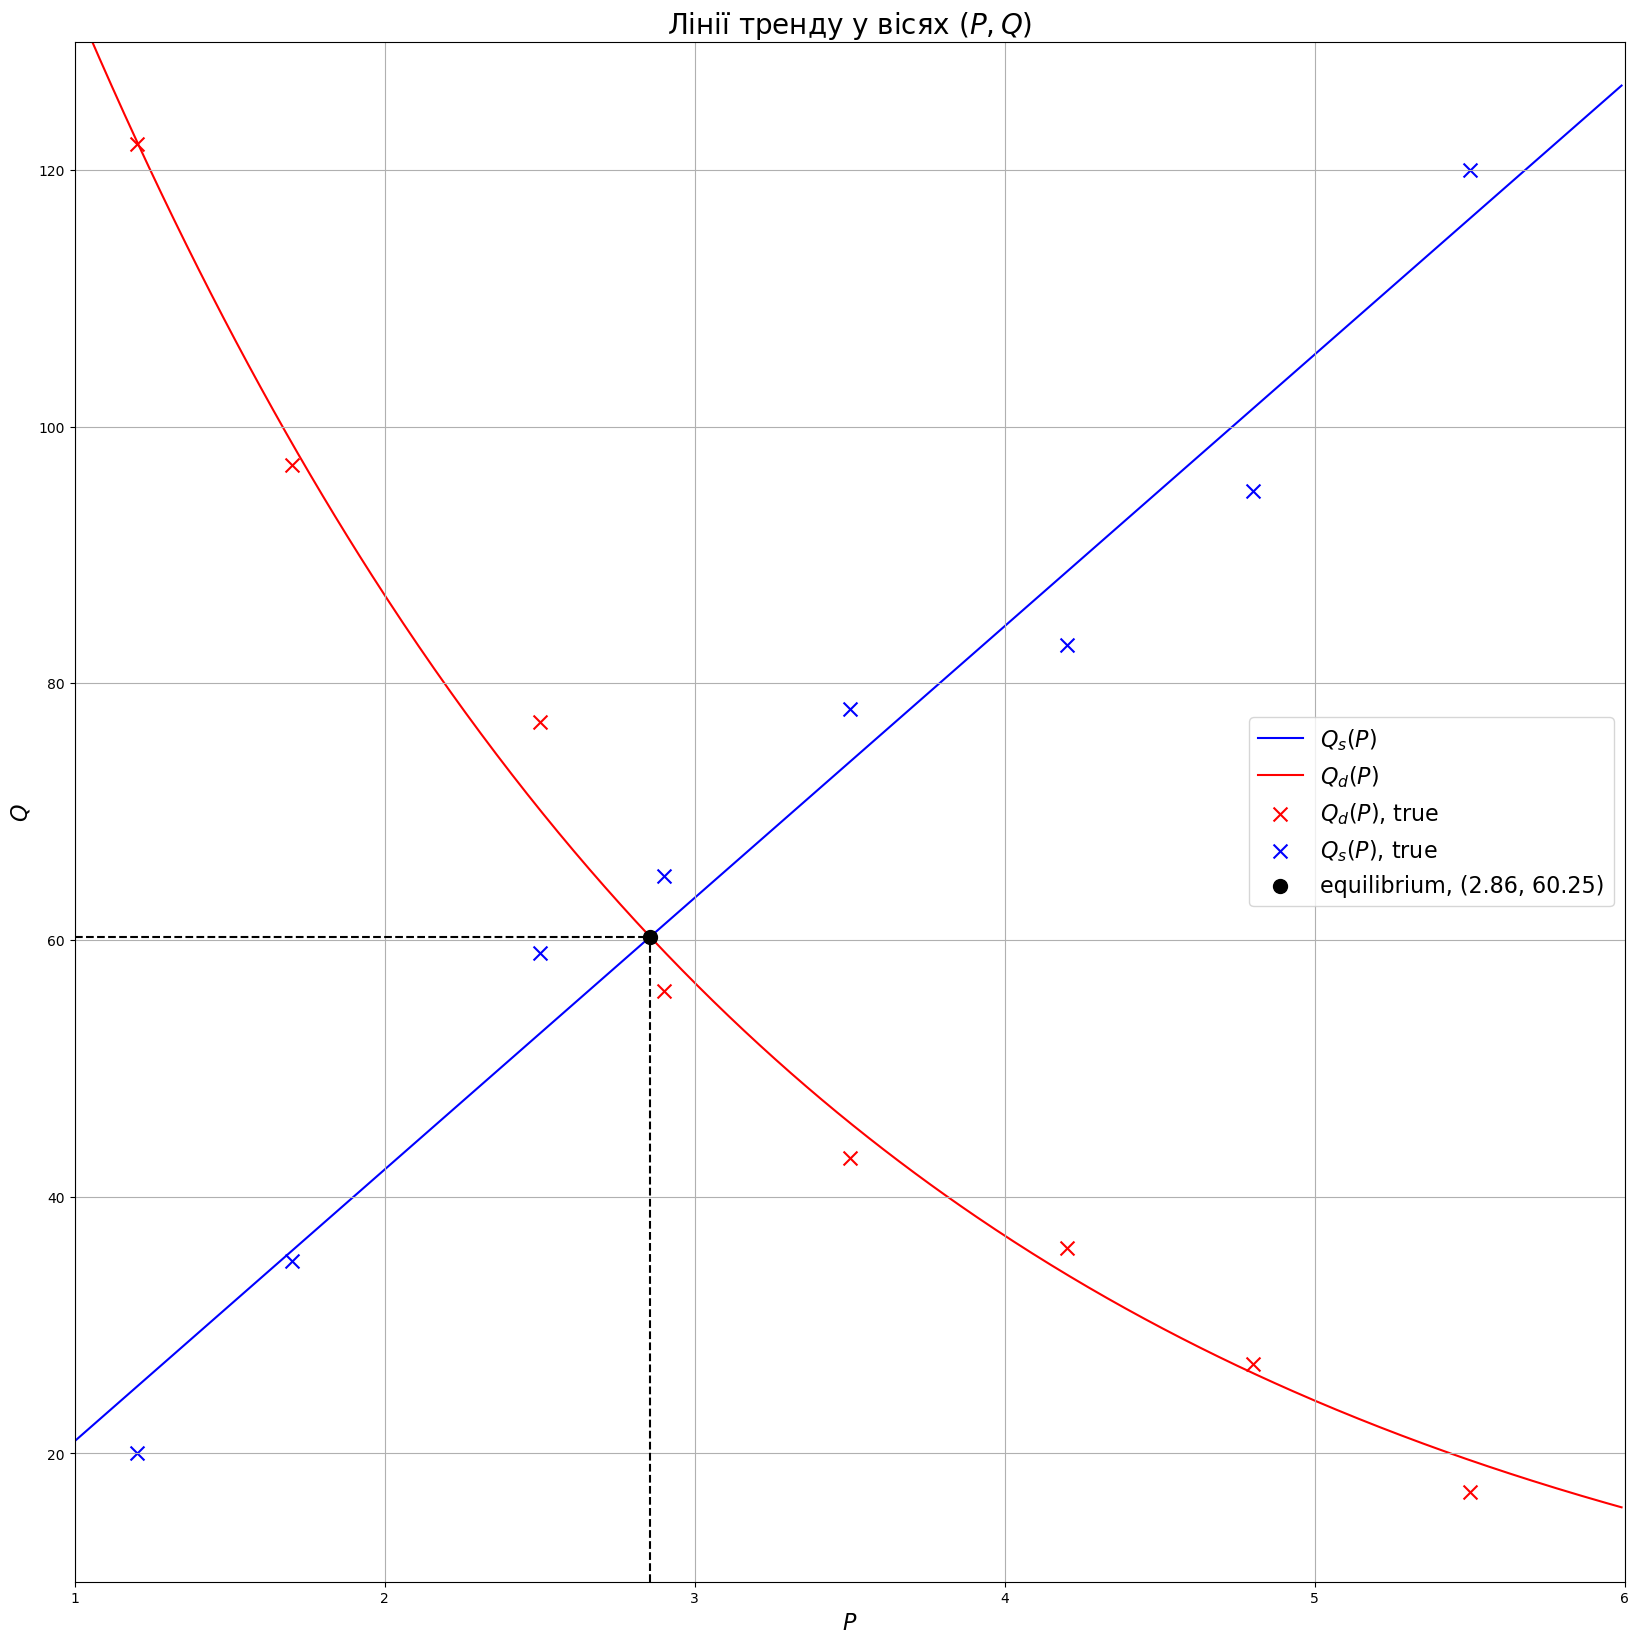
\includegraphics[width=.9\textwidth]{p_q.png}
\end{figure}

\begin{figure}[H]
	\centering
	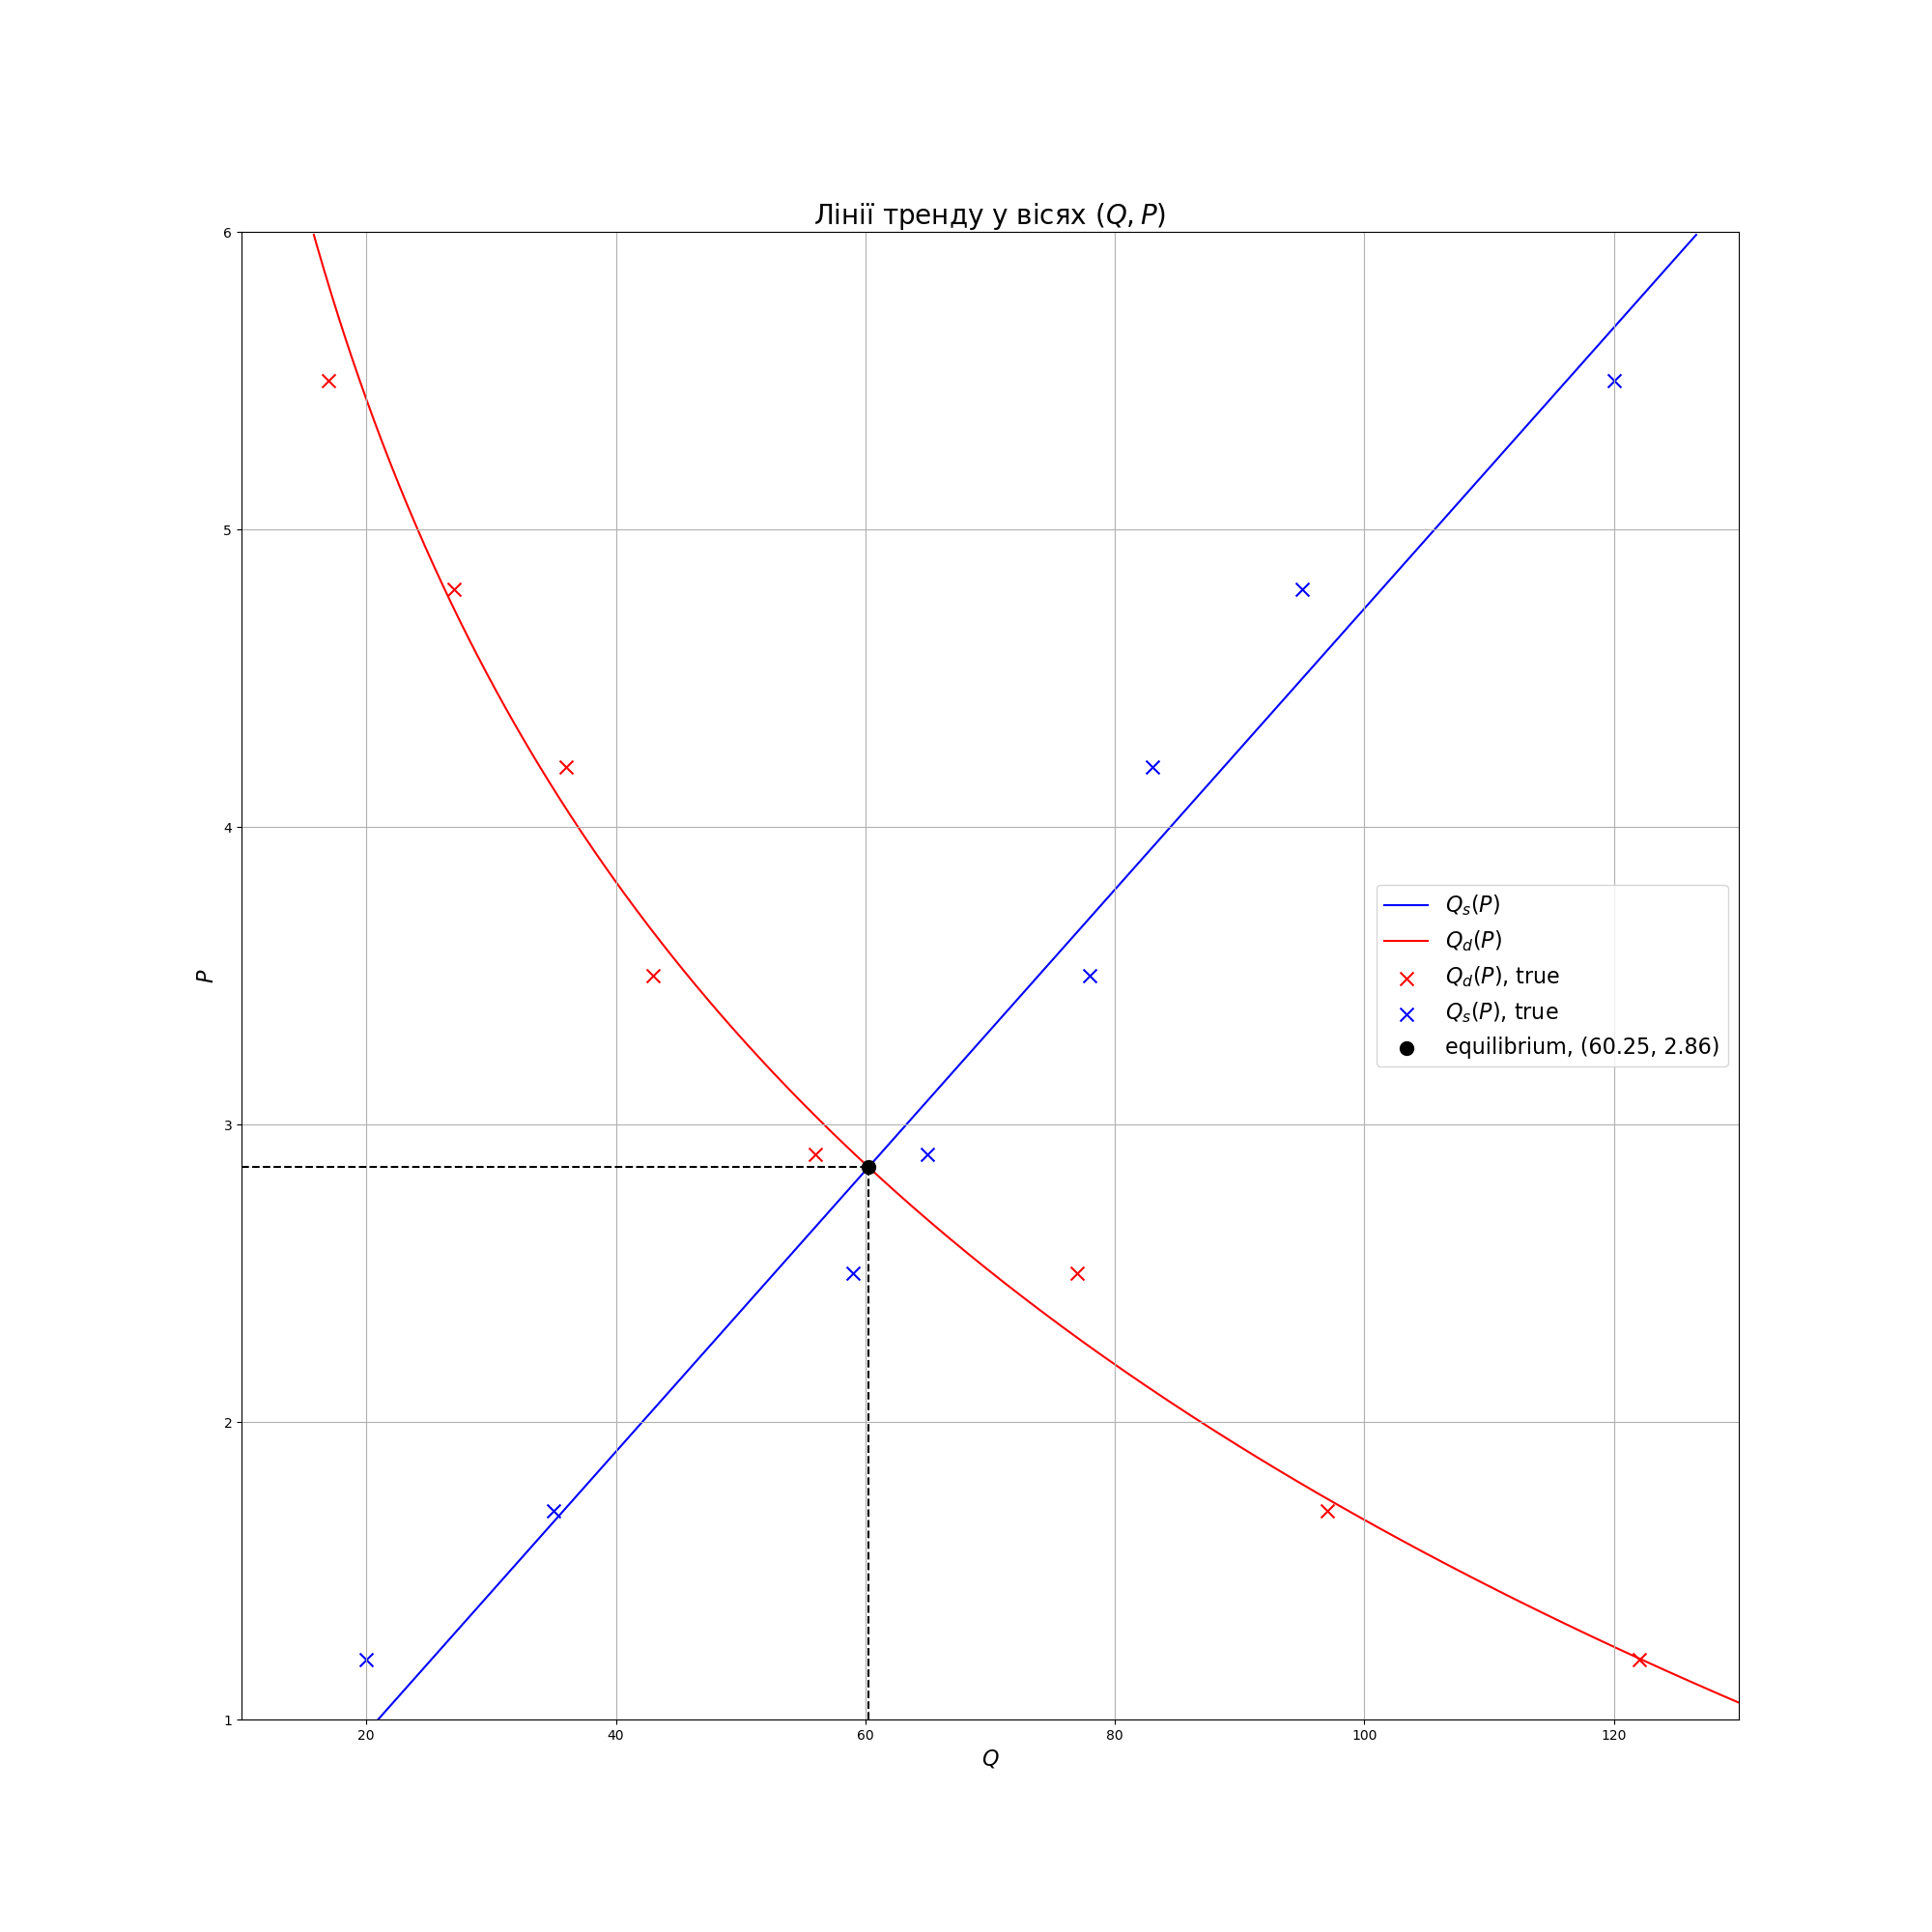
\includegraphics[width=.9\textwidth]{q_p.png}
\end{figure}

Як бачимо, отримані результати відповідають теоретичним очікуванням.

\subsection{Стабільність рівноваги}

З вибраними аналітичними апроксимаційними функціями маємо 
\begin{align*} 
	\left. \left| \dfrac{\diff Q_d}{\diff P} \right| \right|_{P = P^\star} &= \left. \left| -87.7931 \cdot \exp\left\{-0.43 \cdot P\right\} \right| \right|_{P = P^\star} = \\ 
	&= \left. \left( 87.7931 \cdot \exp\left\{-0.43 \cdot P\right\} \right) \right|_{P = P^\star} = \\ 
	&= 87.7931 \cdot \exp\left\{-0.43 \cdot 2.86\right\} \approx 25.6664. \\
	\left. \dfrac{\diff Q_s}{\diff P} \right|_{P = P^\star} &= \left. 21.17 \right|_{P = P^\star} = 21.17.
\end{align*}

Таким чином $\left. \left| \dfrac{\diff Q_d}{\diff P} \right| \right|_{P = P^\star} \approx 25.6664 > 21.17 = \left. \dfrac{\diff Q_s}{\diff P} \right|_{P = P^\star}$, тому рівновага стійка.

\subsection{Вплив дотації}

При введенні дотації (тут $\text{dot} = 0.5$) крива пропозиції зсувається вниз, що дозволяє зменшити рівноважну ціну і збільшити обсяг виробництва.

\begin{figure}[H]
	\centering
	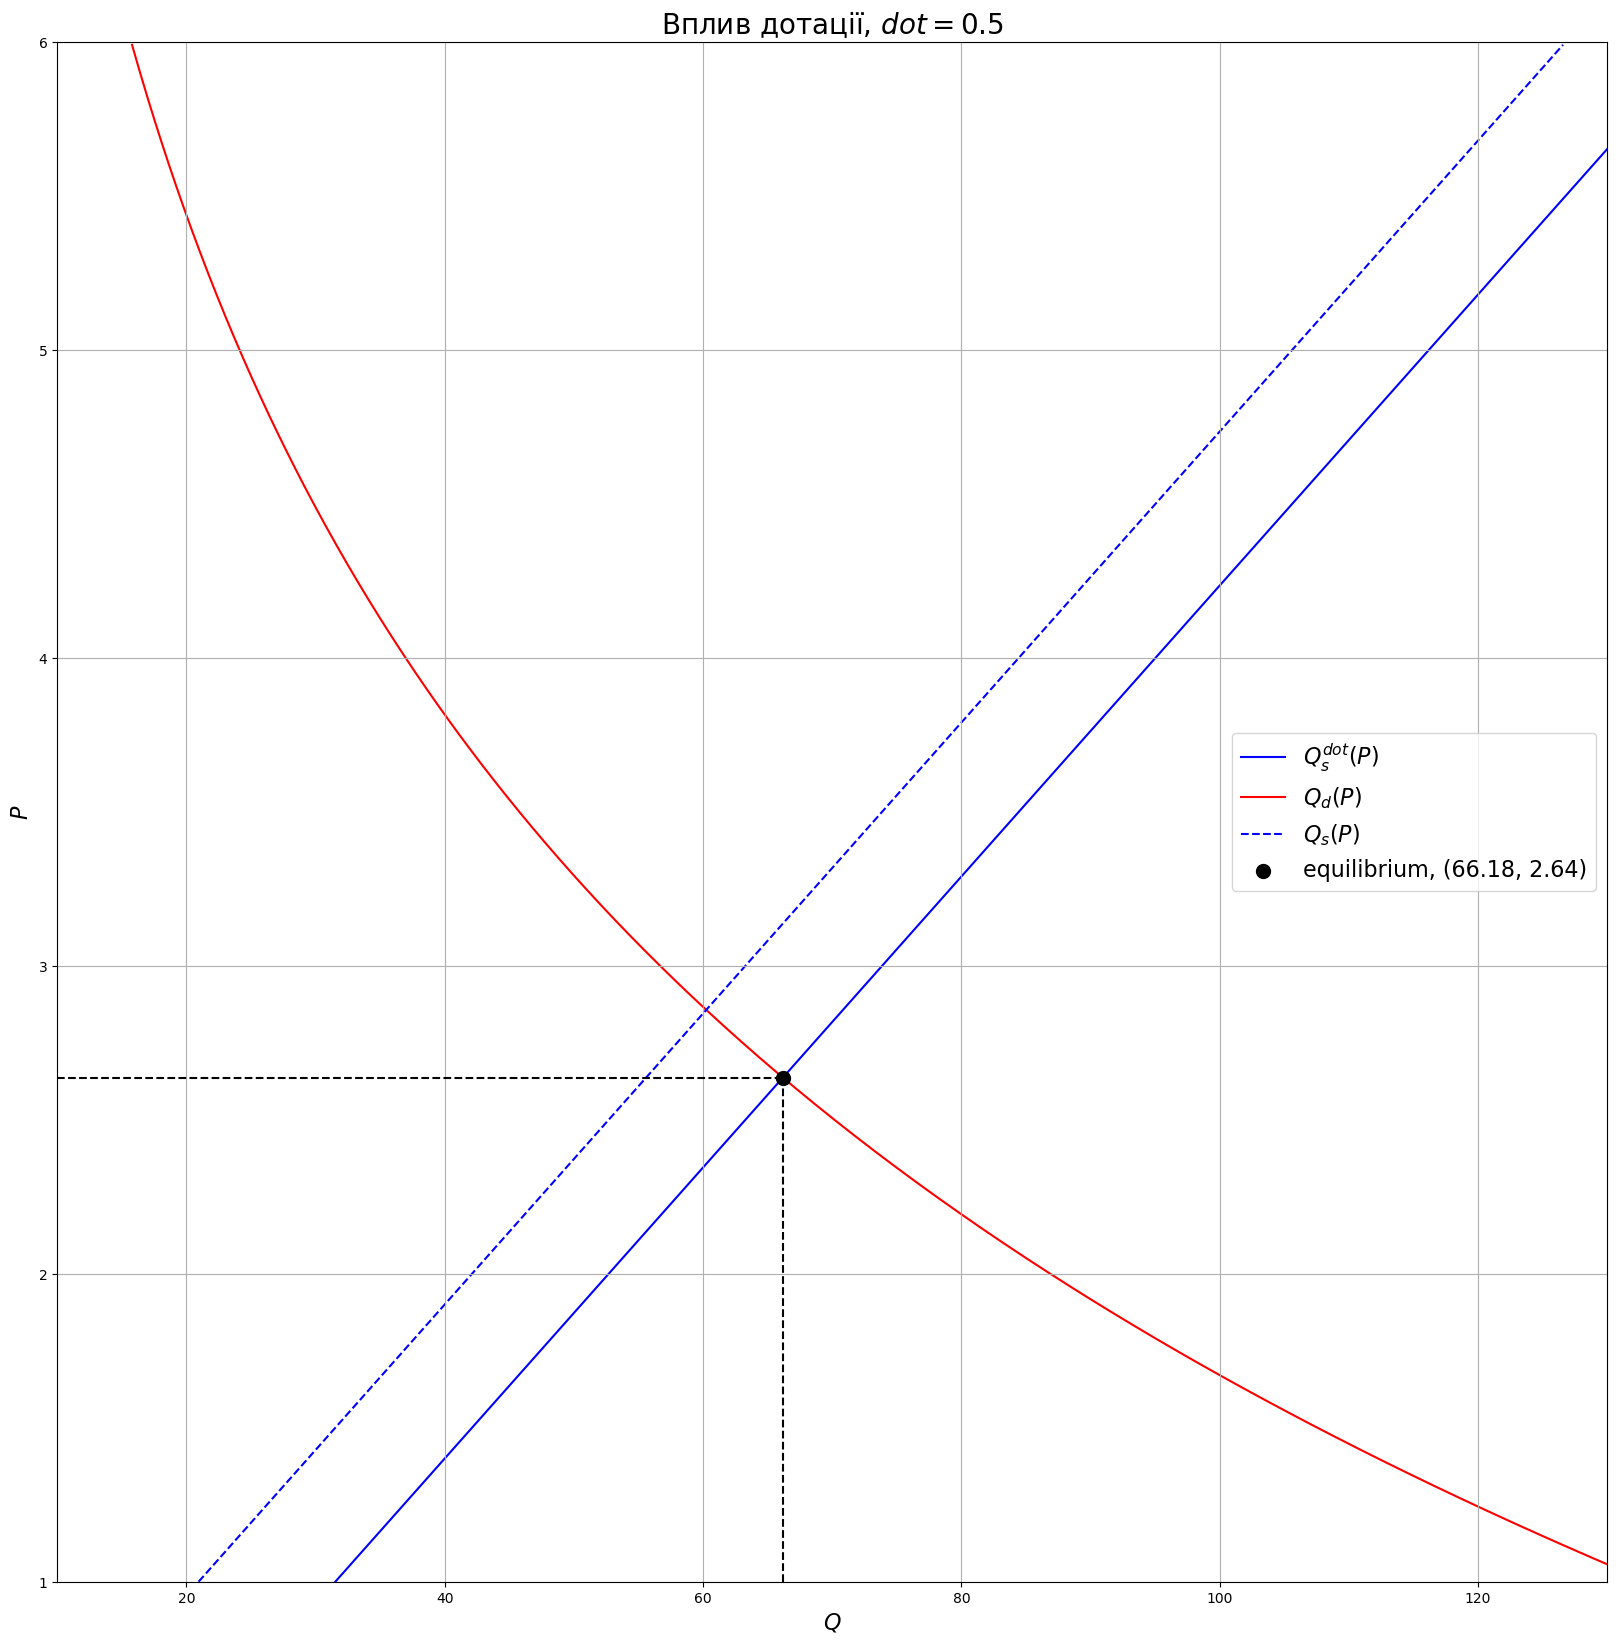
\includegraphics[width=\textwidth]{dotation.png}
\end{figure}

Як бачимо, отримані результати відповідають теоретичним очікуванням.

\end{document}